\startchapter{Capturing the Latent Feature of Power Devices}
\label{chap:latentF}
\section{Introduction}
Power quality meters are expensive devices, which need to place on carefully selected links in the power network. In order to estimate the power quality values on unmonitored links, we use the known power quality values from events reported by meters placed on monitored links. The probabilistic calculation of power quality values on unmonitored links requires the behaviour (latent feature) of each device to be known. We represent the latent feature of a device as a transfer function, which is usually estimated through physical modelling or through the assessment of historical power monitoring data.

In this chapter, we first introduce a latent feature model to capture the behaviour of electric devices in the power network. Using a real power quality dataset, we then demonstrate that the historical data can be used to capture the latent features of a device. We use $k$-fold cross-validation technique to measure the accuracy of latent features we obtain using our dataset. Experimental evaluations show that the captured latent features are consistent.

\begin{figure}[!t]
\center
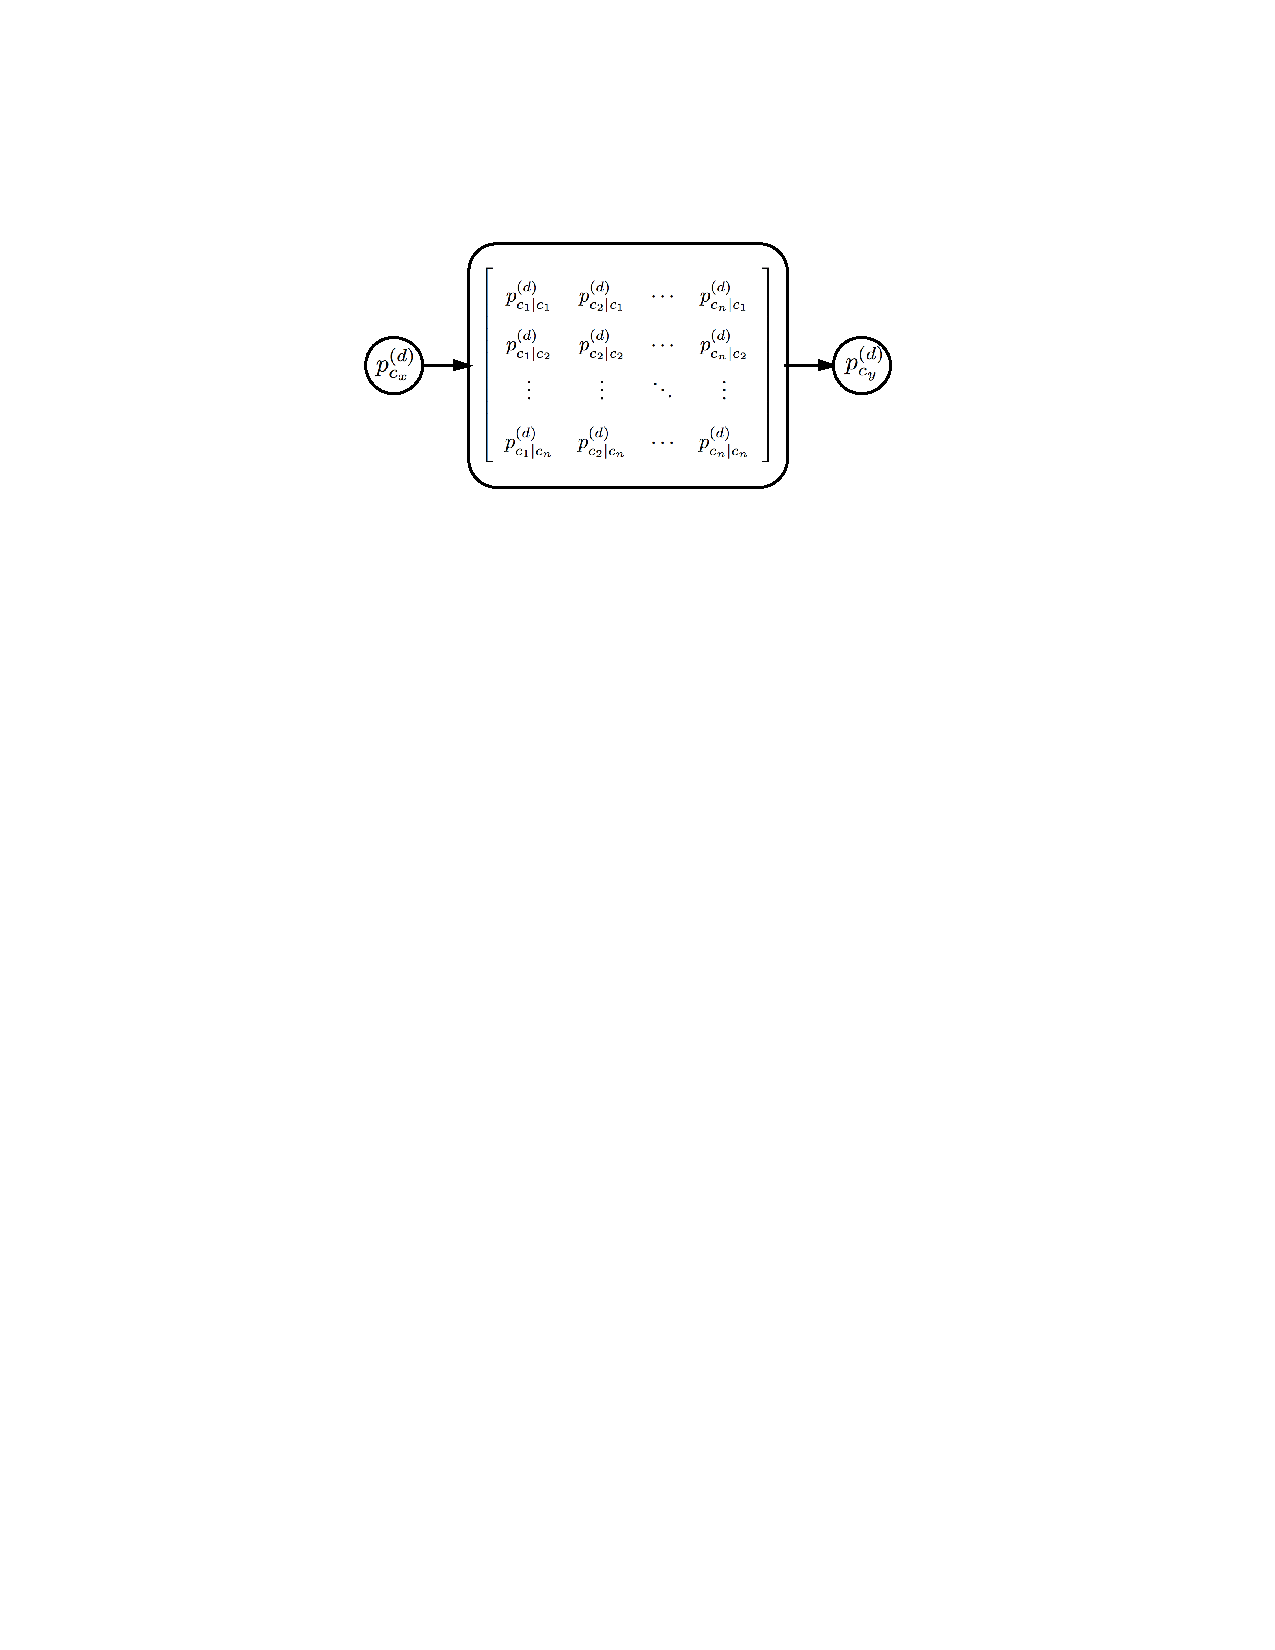
\includegraphics[width=0.75\columnwidth]{latentModel}
\caption{Latent feature model of a device $d$ where the two circles represent the power quality meters at input and output of node $d$; the matrix inside the node $d$ represents the transfer function of the node.}
\label{fig:latentModel}

\end{figure}

\begin{figure}[!t]
\center
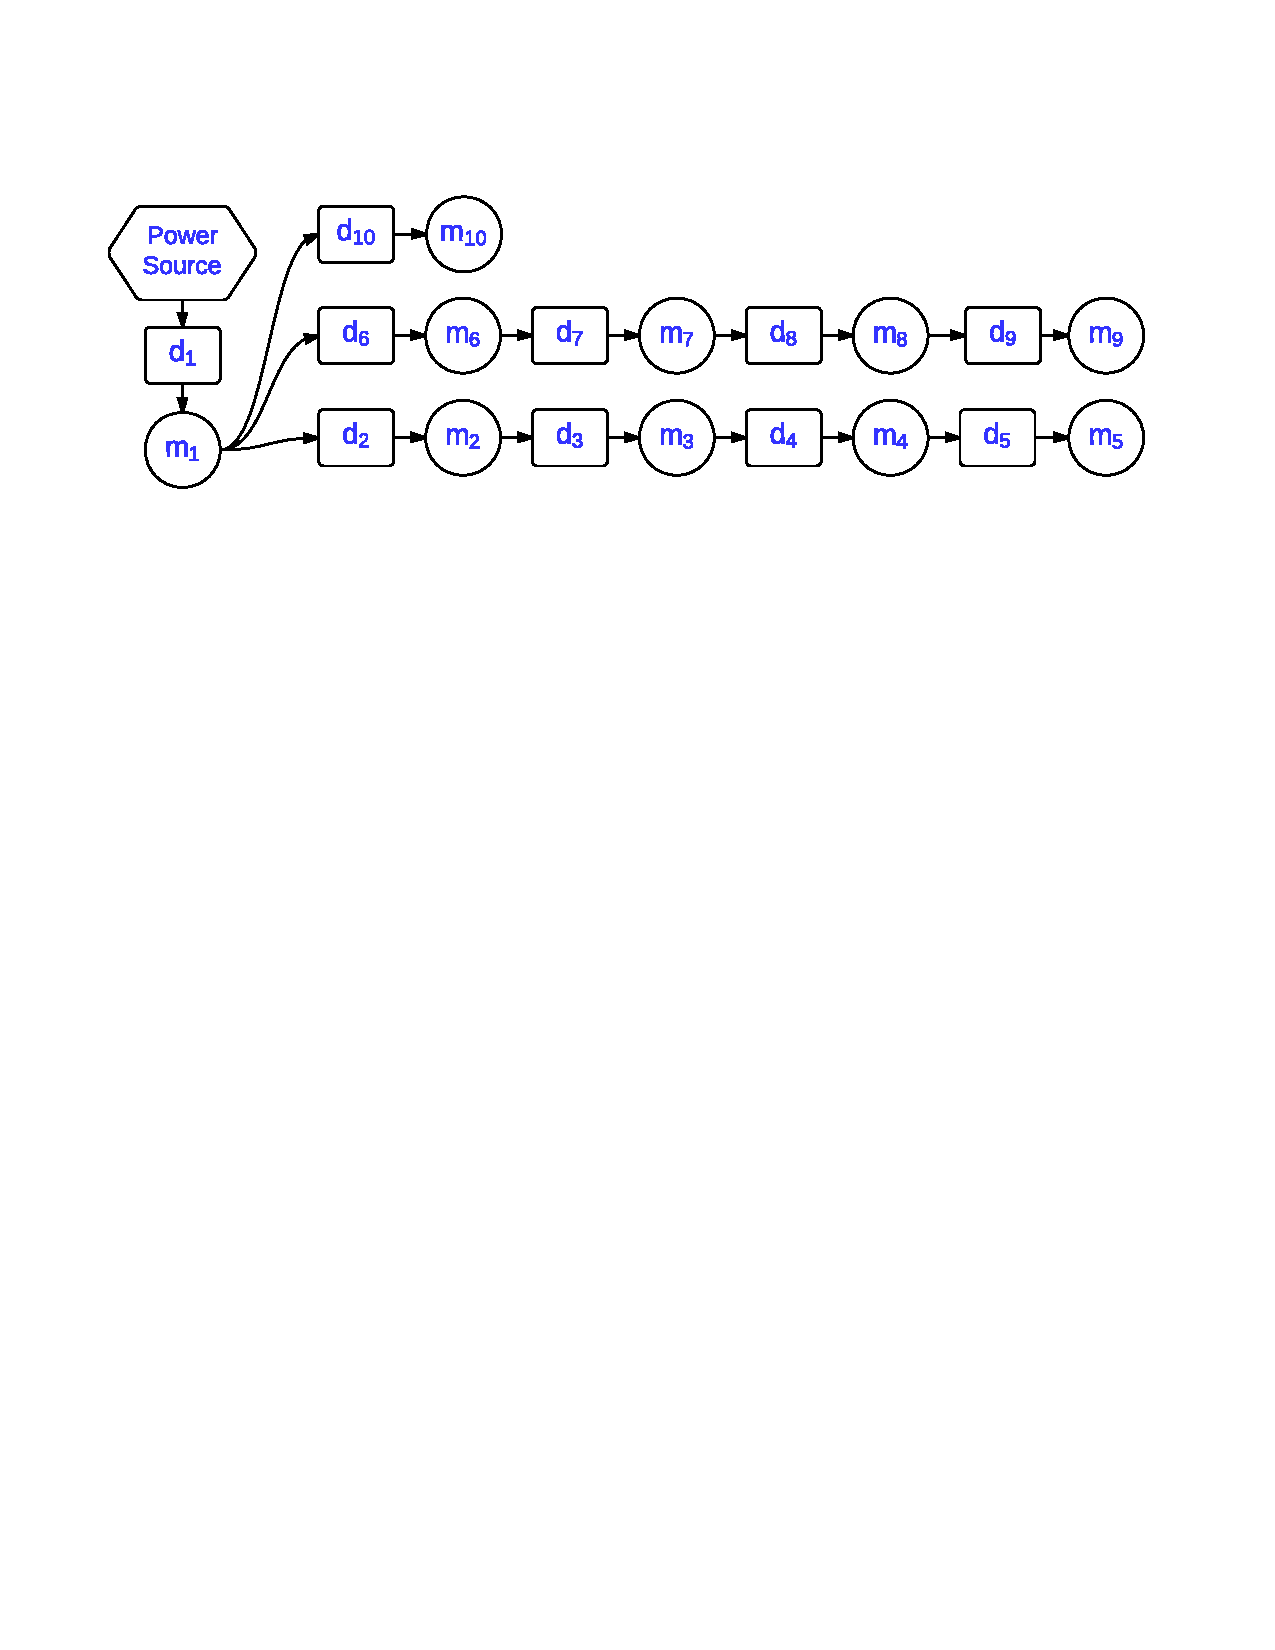
\includegraphics[width=0.98\columnwidth]{pqeNetwork}
\caption{Graph network of power quality meters installed in a power network.}
\label{fig:pqeNetwork}
\end{figure}

\section{The Latent Feature Model}
The latent feature of a device is basically the behaviour of a device in the power network, which can be captured by monitoring the power quality at the input and output links of the device. Based on these power quality readings (events), we model a device behaviour as a transfer function $f{(d)}$. A transfer function of a device is the matrix consisting of real values representing the probabilities that a power quality input $c_x$ is mapped to another power quality $c_y$ at the output link of a device $d$. Figure~\ref{fig:latentModel} shows a sample node (shown as a square box) whose input and output links are monitored (using power quality meters shown in circles) to capture the latent feature $f(d)$. Once the latent feature $f(d)$ is known, we can probabilistically estimate the power quality at links where no power meter is installed.

\section{Power Quality Dataset}
Our power quality dataset was collected at an enterprise power network for a period of four years. For privacy and security reasons, the physical network structure/diagram is omitted. Instead, we represent the topology/positions of the installed smart meters via a graph network as shown in Fig.~\ref{fig:pqeNetwork}. There are a total of $10$ power quality meters (numbered from $m_1$ to $m_{10}$) installed. Each meter reported the power quality events (sag/swell, transient, etc.) to the data collection server via ethernet network. Table~\ref{tbl:perDevFreq} shows the number of events reported by each power quality meter while the positions of the meters are shown in Fig.~\ref{fig:pqeNetwork}.

\begin{table*}[!t]
\caption{Frequency table showing the number of events generated/reported by each power quality meter.}
\centering 
\renewcommand{\tabcolsep}{0.15cm}
\begin{tabular}{|c|c|c|c|c|c|c|c|c|c|c|}
\hline Meter ID & 1 & 2 & 3 & 4 & 5 & 6 & 7 & 8 & 9 & 10\tabularnewline
\hline No. of Events & 1705 & 629 & 756 & 764 & 777 & 282 & 309 & 181 & 44 & 657\tabularnewline
\hline 
\end{tabular}
\label{tbl:perDevFreq}
\end{table*}

\begin{table*}[!t]
\caption{Frequency table showing the number of events classified as IEEE power quality class ($c_i$).}
\centering 
\renewcommand{\tabcolsep}{0.12cm}
\begin{tabular}{|c|c|c|c|c|c|c|c|c|c|c|c|c|c|c|}
\hline Power Quality Class & $c_1$ & $c_2$ & $c_3$ & $c_4$ & $c_5$ & $c_6$ & $c_7$ & $c_8$ & $c_9$ & $c_{10}$ & $c_{11}$ & $c_{12}$ & $c_{13}$ & $c_{14}$\tabularnewline
\hline Number of Events & 3056 & 738 & 1485 & 274 & 144 & 354 & 10 & 11 & 0 & 2 & 8 & 2 & 19 & 1\tabularnewline
\hline 
\end{tabular}
\label{tbl:perClassFreq}
\end{table*}

\begin{table}[!t]
\caption{Sample events from the dataset collected.}
\centering 
\renewcommand{\tabcolsep}{0.15cm}
\begin{tabular}{|c|c|c|c|c|c|c|}
\hline ID & Source & Duration & Magnitude & Severity & Phase  & Type\tabularnewline
\hline 119 & 5 & 0.02 & 292	& 3.19 & V1 & Transient\tabularnewline
 338 & 6 & 1.002 & 147 & 47.1 & V3 & Swell\tabularnewline
 763 & 1 & 0.07 & 84.4 & 1.03 & V3 & Sag\tabularnewline
\hline 
\end{tabular}
\label{tbl:sampleData}
\end{table}

The original power quality events reported by our power quality meters carry detailed information where some of the reported attributes are not directly relevant to power quality monitoring. For instance, we have a large number of branch circuit monitors installed that log every 15 minutes. Second, due to the detailed information content, the size of the raw dataset was about $40$ GB. In order to simplify the format and make the dataset concise and easy to analyze, we transform the reported events into a tabular form consisting of the power quality attributes we used. As a result, there are about $6000$ power quality events recorded in the dataset. Sample events from the dataset are shown in Table~\ref{tbl:sampleData} where: a) each row in the table represents a power quality event; b) the magnitude field represents a percentage of the nominal voltage that the sag or swell reached at its maximum (for instance the number $84$ means that voltage is sagged to $84\%$ of its nominal value, $147$ means that it swelled up by $47\%$ over its nominal value); c) the severity field is a calculated statistic that combines the magnitude, duration and class of an event to provide a ranking variable. 

\begin{table}[!t]
\caption{Sample events classification using IEEE Standard 1159~\cite{IEEE09_1159}.}
\centering 
\begin{tabular}{|c|c|c|c|c|}
\hline Source & Start Time & Duration & Magnitude & IEEE Event Class\tabularnewline
\hline 4 & 733051.9385 & 0.00065 & 127 & $c_1$\tabularnewline
 4 & 733052.9522 & 0.00754 & 146 & $c_2$\tabularnewline
 8 & 733452.0117 & 0.00013 & 132 & $c_1$\tabularnewline
 7 & 733462.7471 & 0.049 & 84 & $c_3$\tabularnewline
 6 & 733488.8235 & 1.002 & 147 & $c_7$\tabularnewline
 6 & 733569.0525 & 0.518 & 79 & $c_6$\tabularnewline
 1 & 733572.9232 & 0.001 & 131 & $c_1$\tabularnewline
 7 & 733589.9307 & 0.016 & 82 & $c_3$\tabularnewline
 6 & 733724.0312 & 7105.48 & 30 & $c_{12}$\tabularnewline
 3 & 733724.1134 & 0.01664 & 233 & $c_4$\tabularnewline
\hline 
\end{tabular}
\label{tbl:sampleClassData}
\end{table}

Using IEEE Standard 1159~\cite{IEEE09_1159}, we classify the power quality events based on the fluctuation of the voltage for a predefined period. There are $14$ different power quality classes defined in the standard, denoted from $c_1$ to $c_{14}$, respectively. Table~\ref{tbl:sampleClassData} shows samples of the events we classify using the IEEE standard where the power quality class is shown in the last column of the table. The frequency of events belonging to the IEEE power quality class ($c_1$ to $c_{14}$) is shown in Table~\ref{tbl:perClassFreq}.

\section{Learning Latent Feature ($f(d)$)}
Using the real-world power quality dataset, we capture the device latent feature as follows:
\begin{itemize}
\item Since most of the PQ events are correlated, i.e., when there is a bad power quality event reported by a meter, the effect may be cascaded and a bad quality event may occur at other links (not necessarily at all links) as well. We identify these cascaded events based on timestamps of the events. When the time stamp is same (or varies by less than a second), we consider them correlated. 
\item For a cascaded event not occurring at a link, we set a nominal PQ value (PQ class $c_{14}$) at that link.
\item We put all the events in a $2$-dimensional array $M(i, j)$ of events where the first dimension of the array represents an event $i$ in the time series while the second dimension represents the corresponding event for each device $j$.
\item The latent feature of a device $d$ is a function giving the probability of an output PQ value at that device given an input value. For every device, we count the frequency of PQ mappings of input to output PQ values. This results in a $14 \times 14$ frequency table ($fr(d)$) for each device $d$. As an example, frequency table for device $d_8$ is shown in Table~\ref{tbl:freqTable}.

\begin{table}[!t]
\caption{A sample frequency table showing the number of events mapped from input power quality $c_i$ to output power quality $c_j$ at device $d_8$.}
\centering 
\begin{tabular}{|cc|llllll|}
\hline
& & \multicolumn{6}{c|}{Output PQ ($c_j$)} \\
& & 1 & 2 & 3 & 4 & 6 & 14 \\
\hline
\multirow{6}{*}{\rotatebox{90}{Input PQ ($c_i$)}}& 3 & 4 & 16 & 4 & 2 & 0 & 113 \\
& 5 & 0 & 0 & 0 & 0 & 0 & 1 \\
& 6 & 0 & 0 & 0 & 0 & 5 & 32 \\
& 7 & 0 & 0 & 0 & 0 & 0 & 2 \\
& 12 & 1 & 0 & 0 & 0 & 0 & 0 \\
& 14 & 47 & 48 & 13 & 24 & 2 & 2122 \\
\hline
\end{tabular}
\label{tbl:freqTable}
\end{table}

\begin{table}[!t]
\caption{A sample transfer function captured at device $d_8$. Rows and columns having all values set to 0 are omitted. }
\centering 
\begin{tabular}{|cc|llllll|}
\hline
& & \multicolumn{6}{c|}{Output PQ ($c_j$)} \\
& & 1 & 2 & 3 & 4 & 6 & 14 \\
\hline
\multirow{6}{*}{\rotatebox{90}{Input PQ ($c_i$)}}& 3 & 0.03 & 0.12 & 0.03 & 0.01 & 0 & 0.81 \\
& 5 & 0 & 0 & 0 & 0 & 0 & 1.00 \\
& 6 & 0 & 0 & 0 & 0 & 0.14 & 0.86 \\
& 7 & 0 & 0 & 0 & 0 & 0 & 1.00 \\
& 12 & 1.00 & 0 & 0 & 0 & 0 & 0 \\
& 14 & 0.02 & 0.02 & 0.01 & 0.01 & 0 & 0.94 \\
\hline
\end{tabular}
\label{tbl:sampleTF}
\end{table}


\item Finally, the transfer function is calculated by dividing every element of the frequency table by sum of the row containing that element, i.e., $f(d, i, j) = fr(d, i, j) / \sum_{k=1}^{14} fr(d, i, k)$. Here, we slightly abuse the notation by using $f(d, i, j)$ to represent the value at the intersection of the $i$-th row and the $j$-th column in matrix $f(d)$. Hence, the transfer function is represented with a matrix. If every element in a row (say $i$-th row) of the frequency table is a $0$, we assume the same probability (i.e., $1/14$) for each element in that row in the transfer function, implying that no knowledge can be learnt from the dataset about the corresponding input event ($c_i$) on this device, and as such we assume the maximum uncertainty on its output events to avoid biased estimation. Table~\ref{tbl:sampleTF} shows a sample transfer function formulated from Table~\ref{tbl:freqTable}.
\end{itemize}

\begin{table}[!t]
\caption{Mean Square Errors (MSEs) in estimated and expected probabilities of the transfer functions.}
\centering 
\begin{tabular}{|cc|lllllll|}
\hline
& & \multicolumn{7}{c|}{Subsets ($k$)} \\
& & 2 & 3 & 5 & 10 & 20 & 50 & 100 \\
\hline
\multirow{9}{*}{\rotatebox{90}{Device ($d_j$)}}
 & 2 & 0.006 & 0.008 & 0.007 & 0.013 & 0.016 & 0.019 & 0.023\\
 & 3 & 0.011 & 0.011 & 0.014 & 0.016 & 0.02 & 0.025 & 0.028\\
 & 4 & 0.015 & 0.014 & 0.016 & 0.019 & 0.021 & 0.028 & 0.031\\
 & 5 & 0.01 & 0.01 & 0.012 & 0.015 & 0.018 & 0.023 & 0.027\\
 & 6 & 0.003 & 0.008 & 0.007 & 0.011 & 0.013 & 0.017 & 0.02\\
 & 7 & 0.019 & 0.018 & 0.023 & 0.019 & 0.021 & 0.023 & 0.024\\
 & 8 & 0.011 & 0.011 & 0.013 & 0.016 & 0.017 & 0.019 & 0.021\\
 & 9 & 0 & 0 & 0 & 0.002 & 0.007 & 0.013 & 0.018\\
 & 10 & 0.002 & 0.007 & 0.006 & 0.01 & 0.013 & 0.017 & 0.021\\
\hline
\end{tabular}
\label{tbl:mse}
\end{table}

\section{Cross-validation of $f(d)$}
We use $k$-fold cross-validation technique to measure the accuracy of latent features we learnt. We partition the dataset (the $2$-dimensional array M formulated above) into $k$ random samples of equal size. Out of the $k$ samples, we use $k-1$ samples to generate a training transfer function and one sample to generate the test transfer function. The cross-validation is repeated $k$ times where each of the k-samples is used exactly once for validation. The $k$ results are then averaged to produce a single estimation for each device.

The Mean-Square Error (MSE) is used to measure the variation of the validation/test function (represented as $f_v(d)$) from its training function (represented as $f_t(d)$).  The MSE is calculated as: \[mse = \sum_{i=1}^{14} \sum_{j=1}^{14} \mid f_v(d, i, j) - f_t(d, i, j) \mid / (i \times j).\]

We use $k=2,3,5,10,20,50,100$ in our experiments. As the value of $k$ increases, the number of events in the test data set reduces. For small value of $k=2$, we divide the entire dataset in $2$ sub-sets of equal size where one is used for training and the other is used for testing.

Table~\ref{tbl:mse} shows the MSEs for all devices in the network at various sample sizes where it can be clearly seen that the values are slightly increasing with increase in the value of $k$. At $k=100$, the largest value is $0.0285$, i.e., in the worst case, the error between the trained and tested values is $2.8\%$ on average. The small error values suggest that a device behaviour (latent feature) can be captured accurately with historical PQ data from power quality meters.

\section{Conclusion}
In this chapter, we proposed a device latent feature model which learns a device transfer function from real data. The device transfer function is needed to estimate the power quality values on unmonitored links in the power gird. In order to validate the proposed model, We used a real power quality dataset collected by Schneider Electric Inc. in a power grid in Canada. We demonstrated that the historical data can be used to capture the latent features of a device. The $k$-fold cross-validation technique was used to measure the accuracy of latent features we obtained using our dataset. Experimental evaluations showed that the captured latent features are consistent. The latent features learnt in this chapter are used by our meter placement algorithms proposed in Chapter~\ref{chap:meterPlacement}.